\chapter{Porovnání integračních metod}
V této kapitole alespoň zběžně porovnáme implementované integrační metody. Protože potencionálního uživatele by mohlo zajímat, kterou metodu by měl použít pro co nejpřesnější ale i nejrychlejší výsledek.

Srovnání bude probíhat nejdříve na případu kruhového pohybu. Důvod je ten, že je to podobný případ jako gravitace a také už pro něj máme vyřešenou implicitní verzi Eulerovy metody. Budeme hodnotit přesnost, stabilitu v závislost na $ \Delta t $ a výpočetní složitost.

V dalších sekcích už nebudeme metody znovu vysvětlovat, pouze se odkážeme na odpovídající kapitoly.

\section{Kruhový pohyb}
Zdrojové kódy použitých metod, které byly použity k získání dat, jsou dostupné v souboru \texttt{Source/stabilita.cpp}. Dále je zde soubor \texttt{plot.gp} pomocí něhož a gnuplotu
\footnote{\url{http://www.gnuplot.info/}}
 vznikly všechny obrázky.
\subsection{Teorie}
Pohyb po kružnici v rovině můžeme zapsat rovnicí \eqref{eq:kruh}, kde $\omega$ je úhlová rychlost. Což je také řešení diferenciální rovnice \eqref{eq:kruhDif}
\begin{align}
\label{eq:kruh}
\boldsymbol{u}(t) &= (x,y)(t)=(cos(\omega t),sin(\omega t))\\
\label{eq:kruhDif}
\ddot{\boldsymbol{u}}(t)&=-\omega^2u(t) \quad \boldsymbol{u}(0)=(1,0) \quad \dot{\boldsymbol{u}}(0)=(0,1)
\end{align}
V dalších částech zvolíme $ \omega = 1 $.
\subsection{Explicitní Euler}
Explicitní Eulerovu metodu jsme si představili v úvodní teorii \ref{sec:numReseni}. Zde jen připomeneme, že si opět rovnici \eqref{eq:kruhDif} rozdělíme na dvě rovnice prvního řádu a integrujeme je samostatně. Výsledky jsou zobrazeny v grafu na obrázku \ref{fig:explicitEuler}, z něhož je vidět, že explicitní metoda diverguje od správného řešení pro libovolné $ \Delta t $ Což není moc překvapivé, protože považuje derivaci na integračním oboru za konstantní, což je na počátku tečna procházející bodem (1,0) a tím dojde vždy k posunu směrem ven z kružnice. Takže tato metoda není moc vhodná pro naši simulaci, proto není ani implementována.
\begin{figure}
	\caption{Explicitní Eulerova metoda $ t\in [0,10] $}
	\label{fig:explicitEuler} 
	\centering
	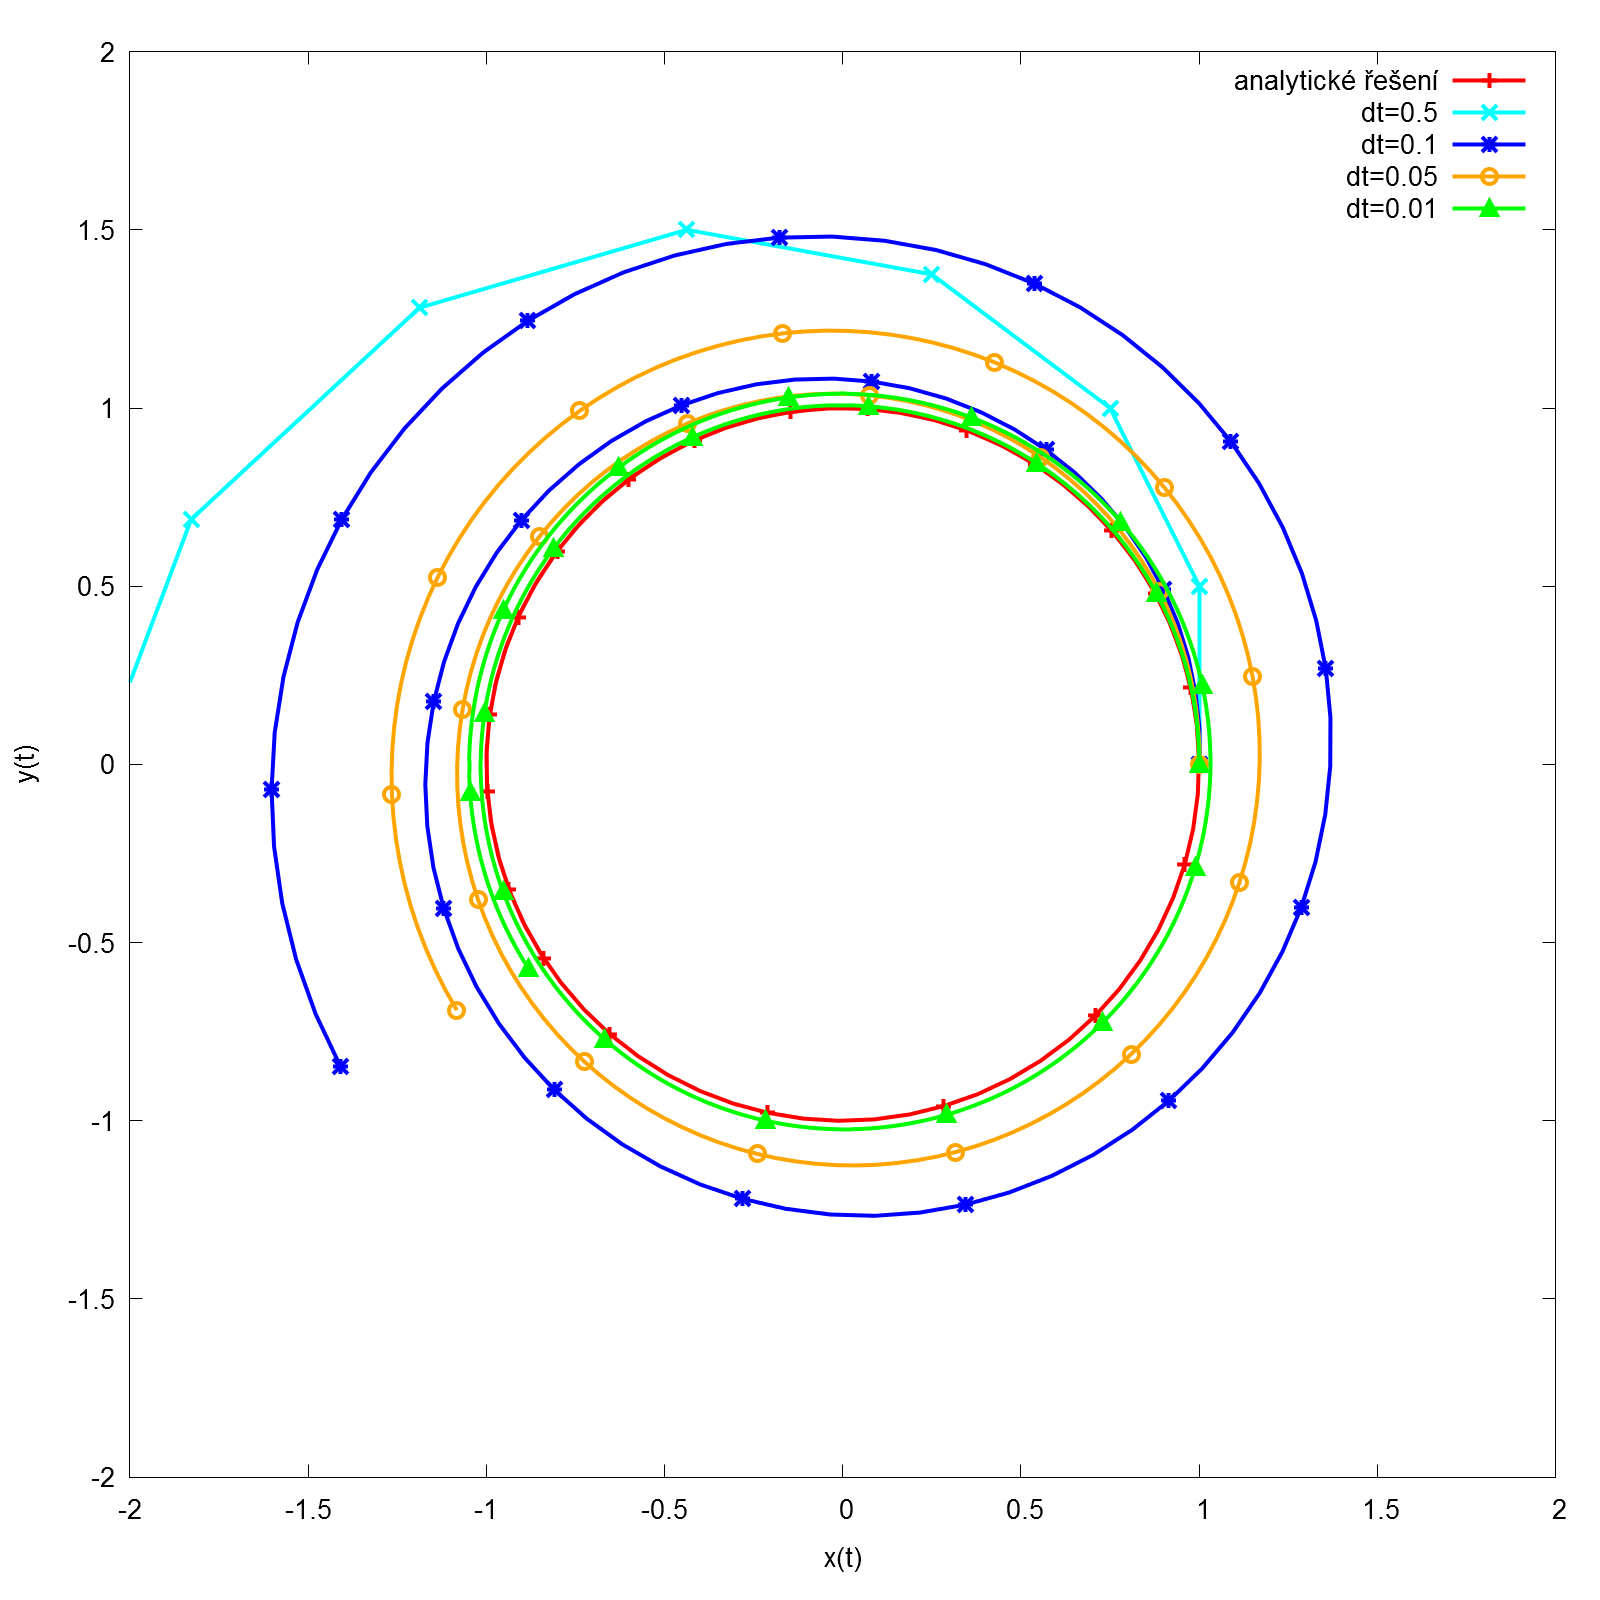
\includegraphics[width=\linewidth]{Figs/explicitEuler}
\end{figure}
\subsection{Implicitní Euler}
Implicitní Eulerova metoda byla ukázána v části \ref{sec:implEuler} i s řešením jedné rovnice \eqref{eq:implicitEuler}, které můžeme použít, neboť platí, že $ k=-\omega^2 $. 
Bohužel ani tato metoda není ideální jak ukazuje obrázek \ref{fig:implicitEuler}. Dochází zde k opačnému jevu, což je způsobeno tím, že integrace probíhá po tečně v čase $ t+\Delta t $, což vede k posunu směrem do kružnice. Implicitní metoda nebyla použita, protože se z naší soustavy \eqref{eq:soustava} nedá jednoduše vyjádřit a stejně by nepřinesla užitečné výsledky.
\begin{figure}
	\caption{Implicitní Eulerova metoda $ t\in [0,10] $}
	\label{fig:implicitEuler} 
	\centering
	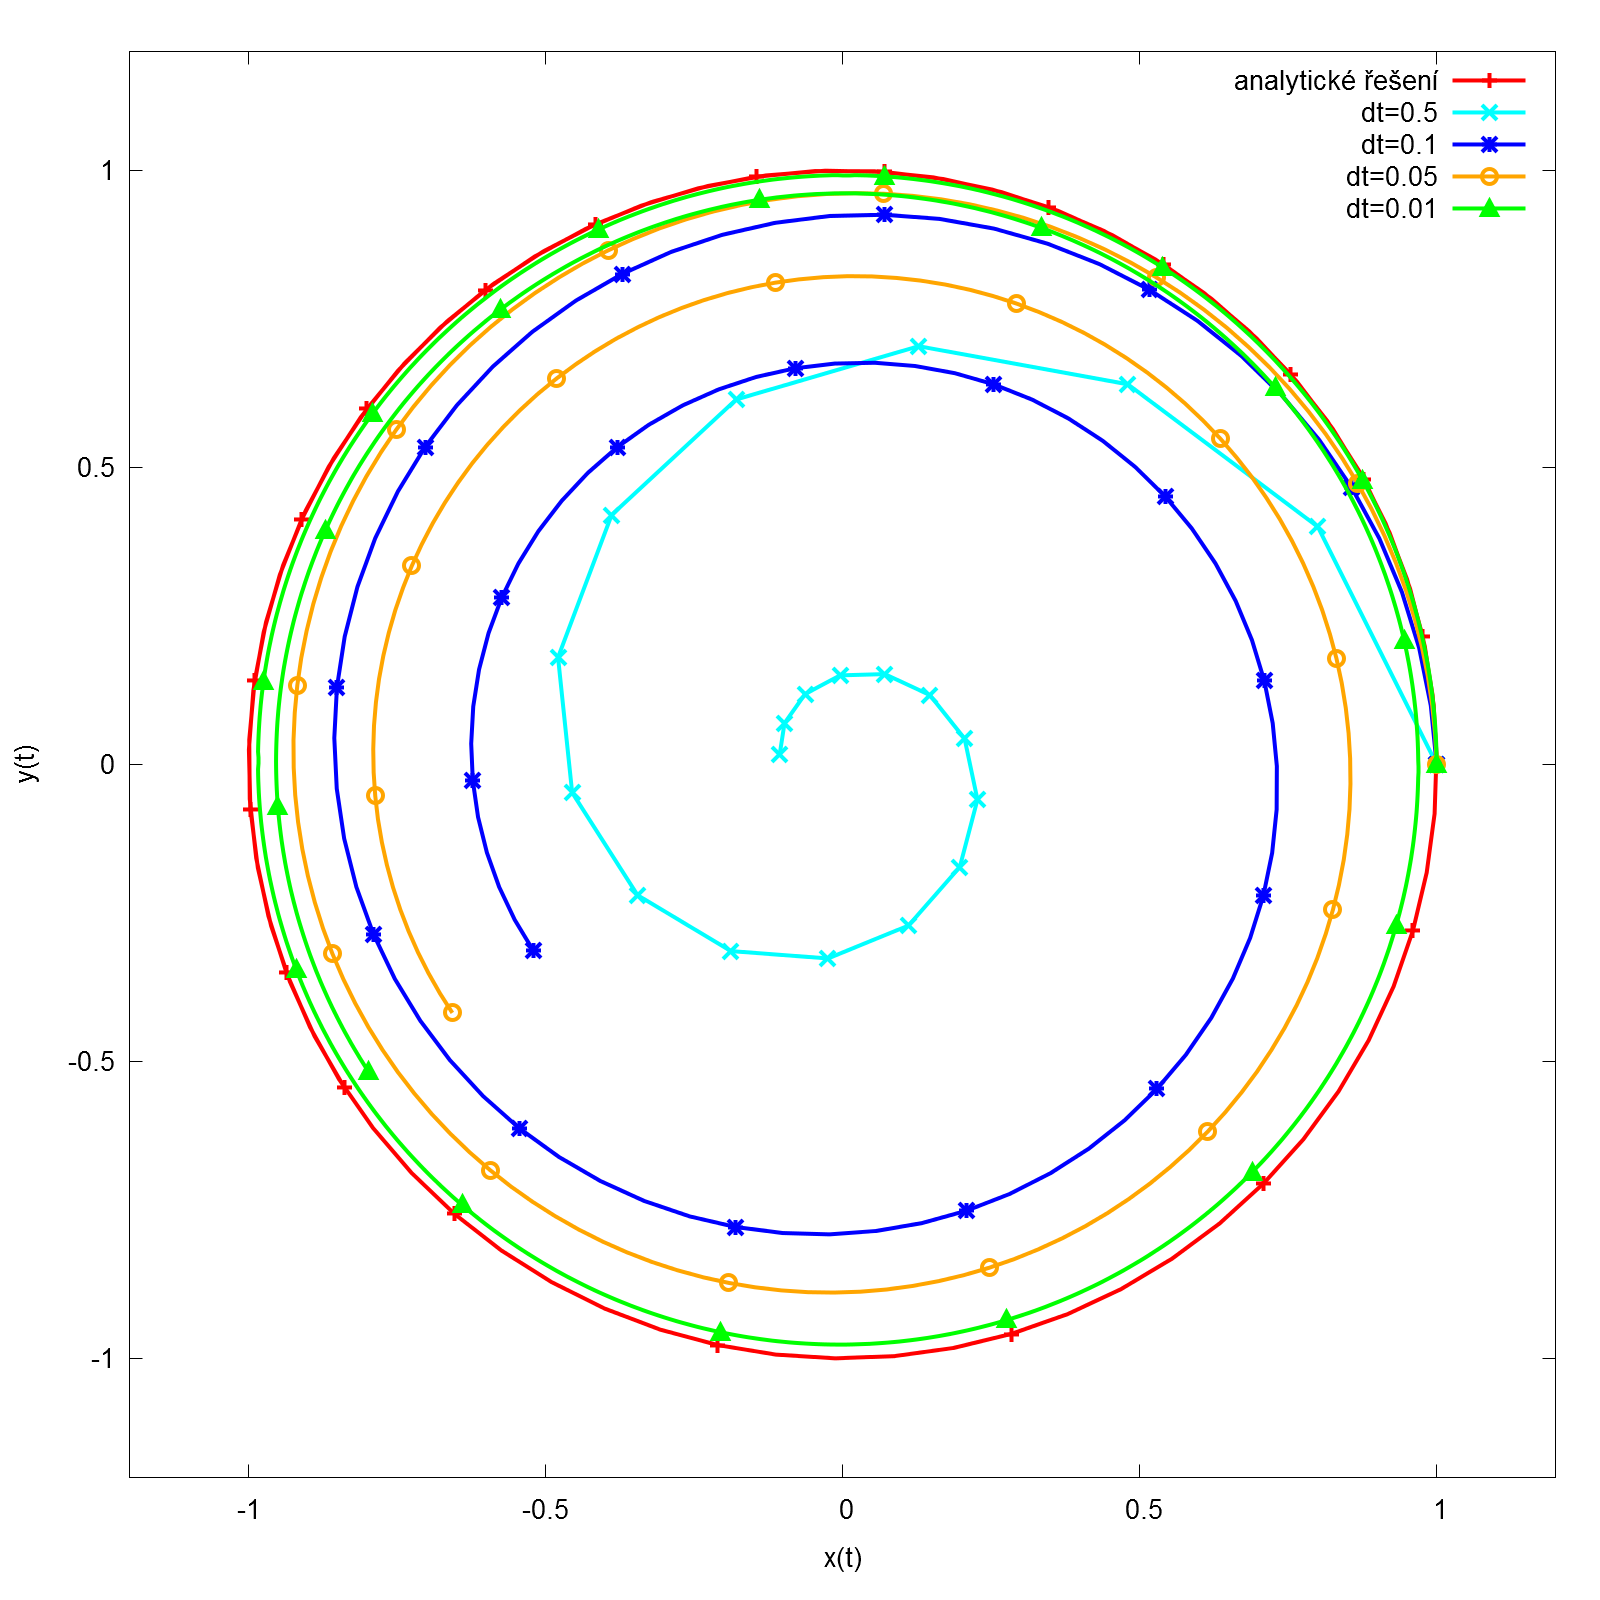
\includegraphics[width=\linewidth]{Figs/implicitEuler}
\end{figure}
\subsection{Semi-implicitní Euler}
Tato metoda je navrhnuta také v části \ref{sec:implEuler} jako jednodušší řešení implicitní verze. Z obrázků \ref{fig:semiImplEuler} a \ref{fig:semiImplEulerStab} je vidět, že je tato metoda navíc stabilní i pro větší $ \Delta t $, ale pro ně není už moc přesná.

\begin{figure}
	\caption{Semi-implicitní Eulerova metoda $ t\in [0,10] $}
	\label{fig:semiImplEuler} 
	\centering
	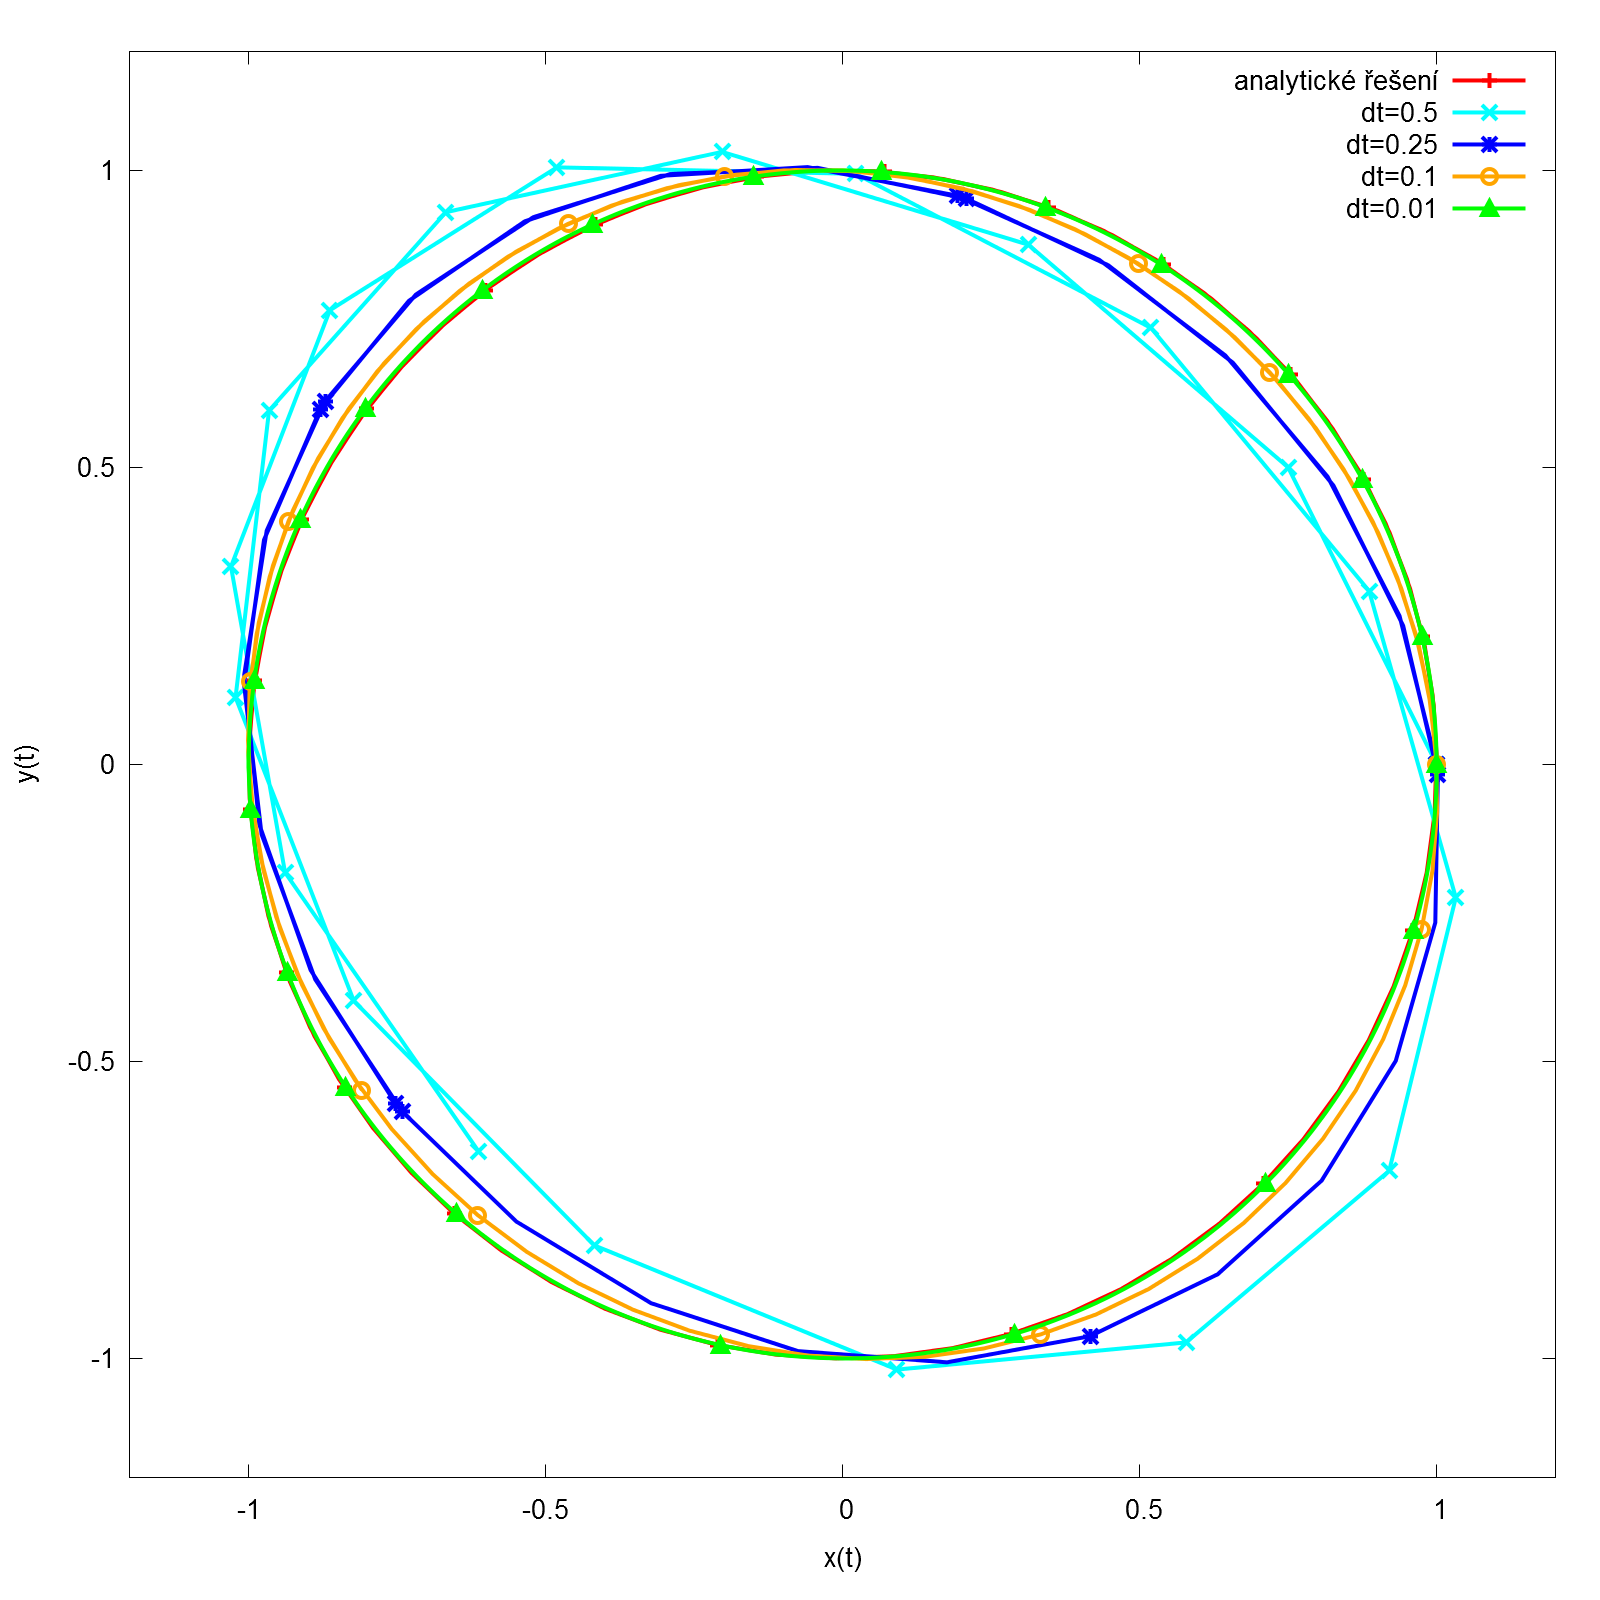
\includegraphics[width=\linewidth]{Figs/semiImplEuler}
\end{figure}
\begin{figure}
	\caption{Semi-implicitní Eulerova metoda $ t\in [0,100] $}
	\label{fig:semiImplEulerStab} 
	\centering
	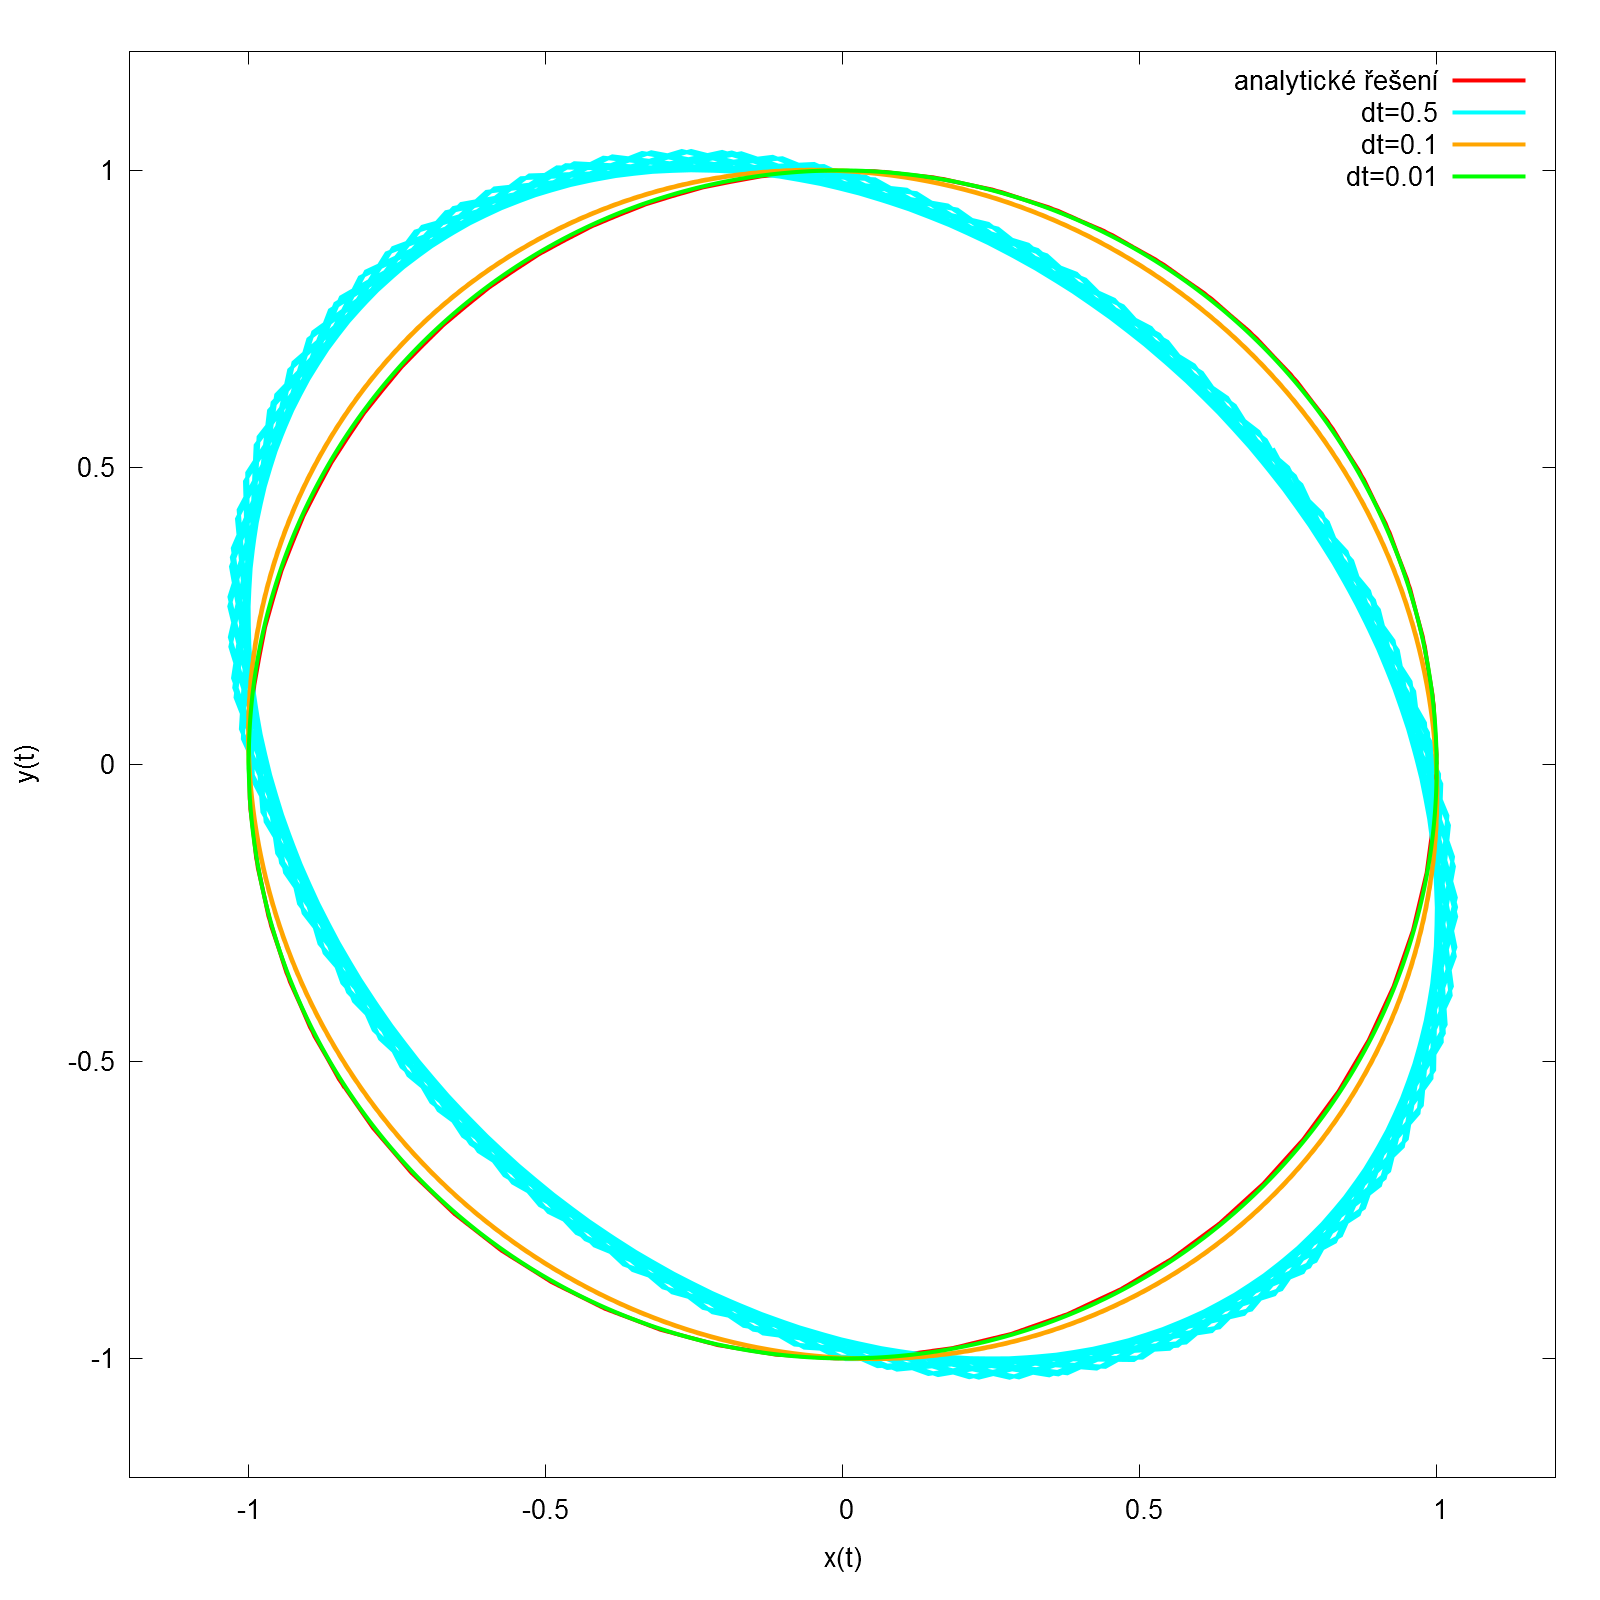
\includegraphics[width=\linewidth]{Figs/semiImplEulerStab}
\end{figure}
\subsection{RK4}
Poslední implementovaná metoda je RK4, která je popsána v sekci \ref{sec:implRK4}. Její přesnost zachycují obrázky \ref{fig:RK4} a \ref{fig:RK4Stab}. Tedy už při $ \Delta t=0.1 $ se jedná o velmi stabilní metodu a je přesnější než semi-implicitní metoda . Ale naopak pro vyšší  $ \Delta t$ stabilní není.
\begin{figure}
	\caption{RK4 metoda $ t\in [0,10] $}
	\label{fig:RK4} 
	\centering
	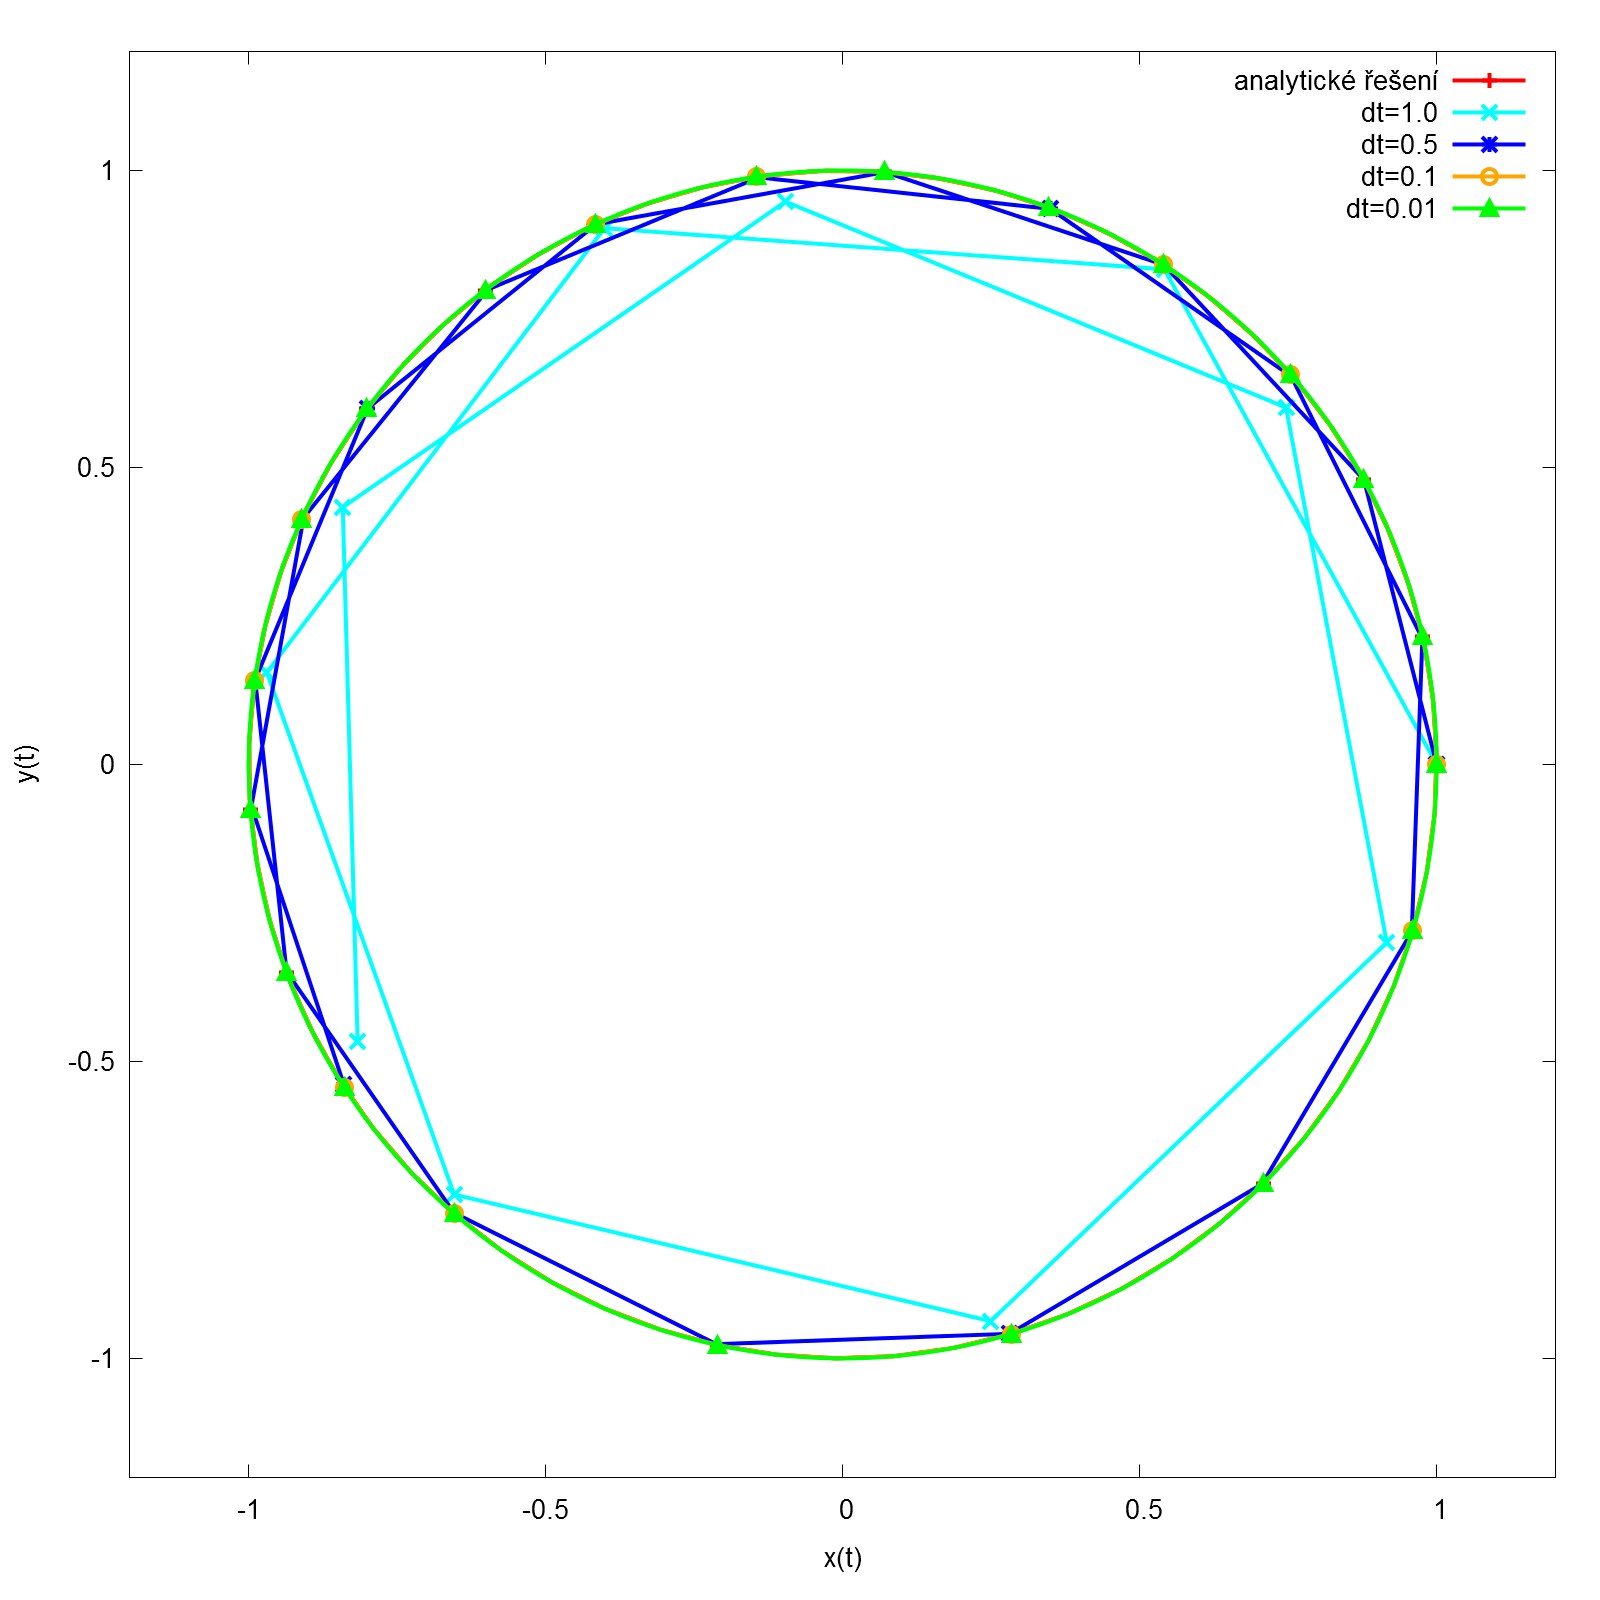
\includegraphics[width=\linewidth]{Figs/RK4}
\end{figure}
\begin{figure}
	\caption{RK4 metoda $ t\in [0,10] $}
	\label{fig:RK4Stab} 
	\centering
	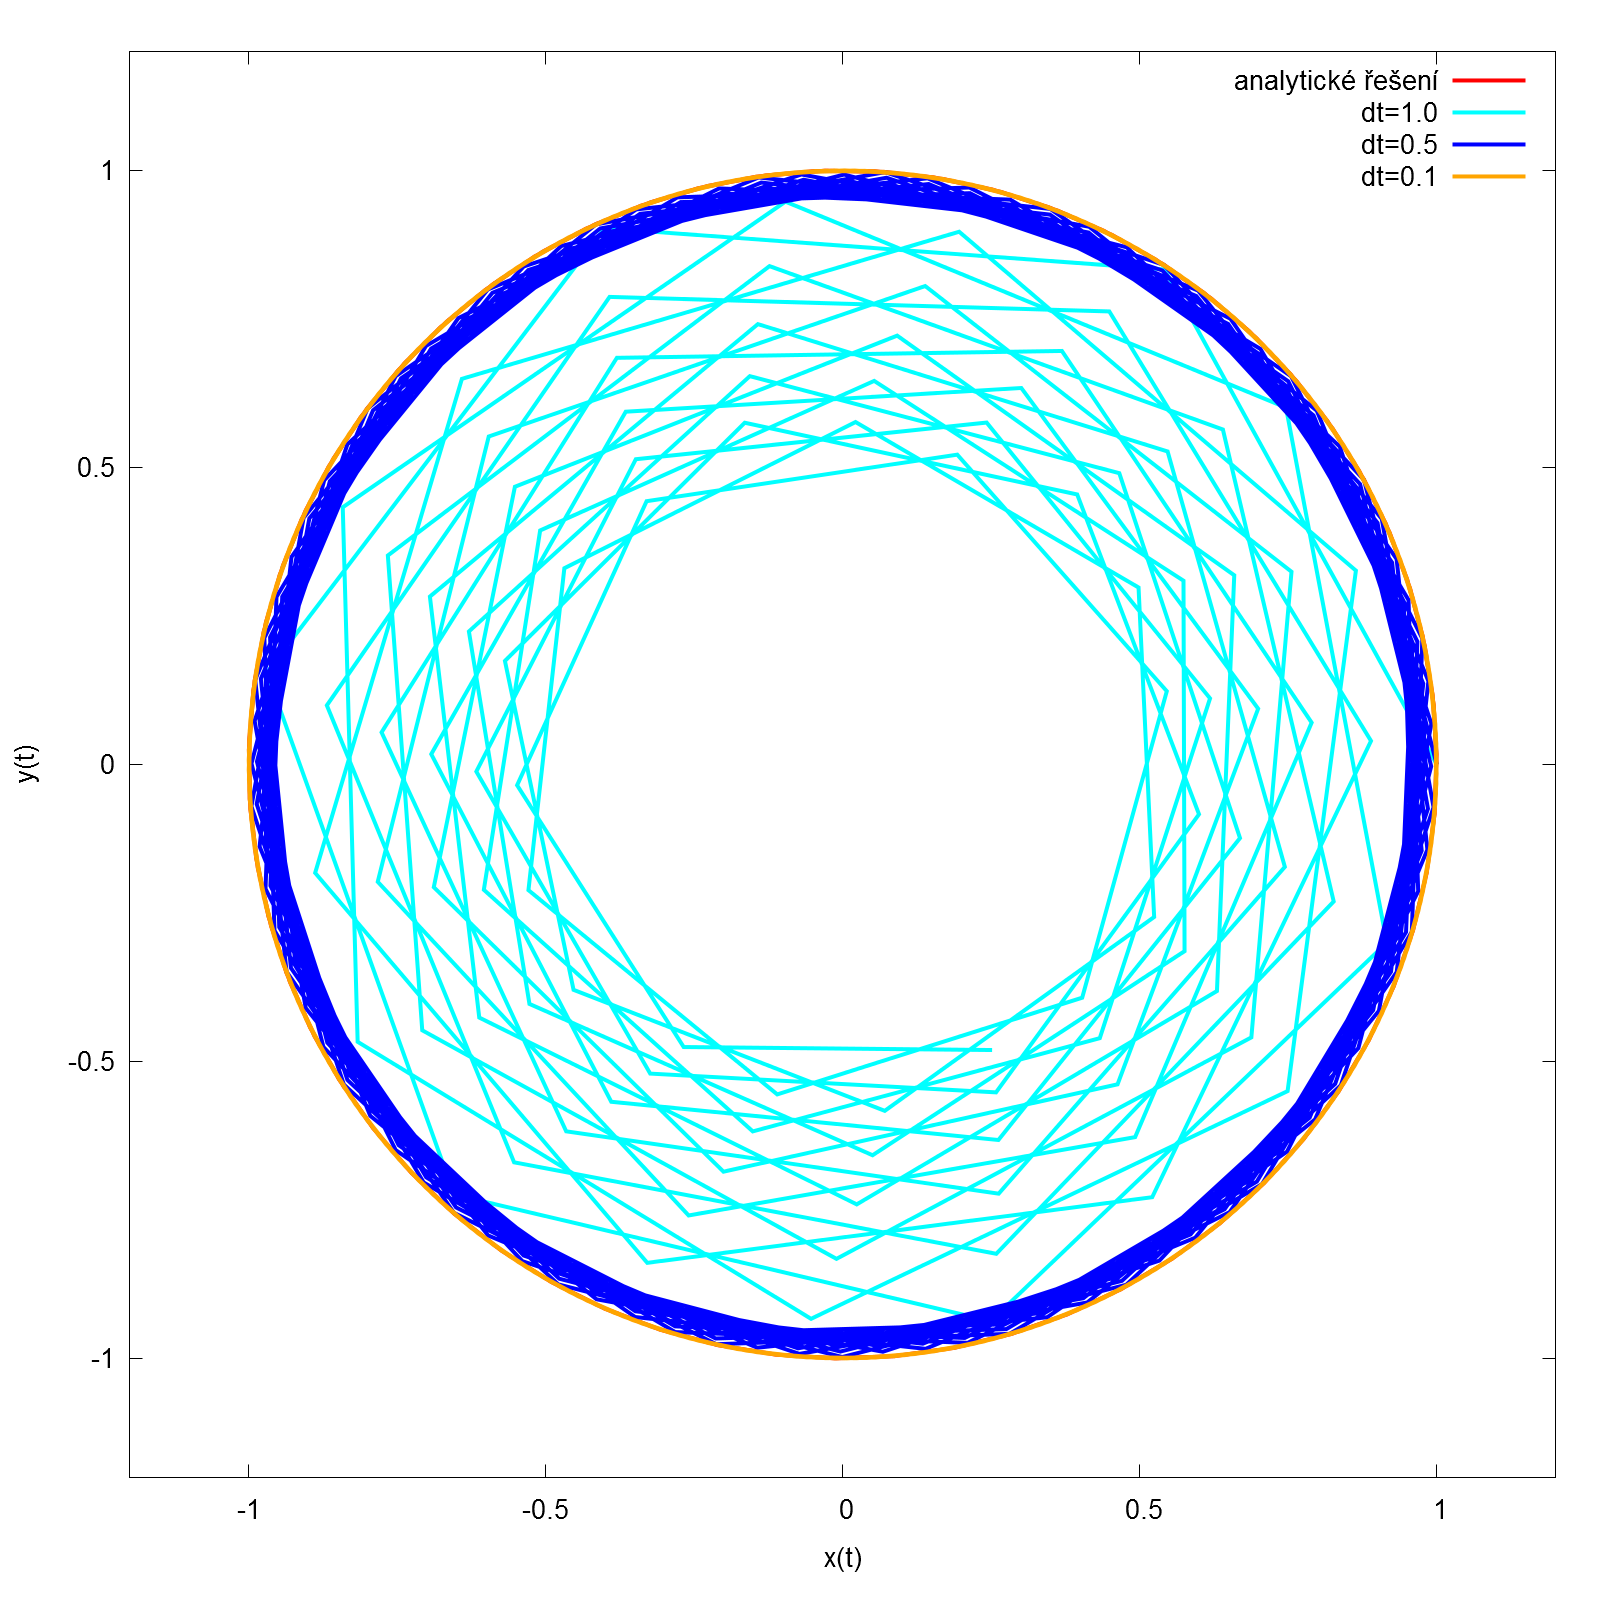
\includegraphics[width=\linewidth]{Figs/RK4Stab}
\end{figure}
\section{Sluneční soustava}
Pojďme se ještě podívat na srovnání stability semi-implicitní a RK4 metody na příkladu naší Sluneční soustavy. Jako indikátor stability použijeme stabilitu oběžných drah měsíců, protože ty mají nejkratší oběžné doby a nestabilita se zde projeví jako první. Samozřejmě toto je pouze nutná a ne postačující podmínka správné simulace, ale pro běžné porovnání by mohla stačit. Naměřené údaje jsou uvedeny v tabulce \ref{tab:stab}. Vyšší hodnoty nejsou podstatné, protože se zde ve velké míře projeví nepřesnost, která vyvolá nestabilitu systému. Každopádně to ukazuje, že semi-implicitní Eulerova metoda je stabilnější, což i trochu naznačovaly obrázky u kruhového pohybu, ale také obrázek \ref{fig:semiImplEulerStab} ukazuje stabilní, avšak nesprávný \uv{orbit}. Na druhou stranu obrázek \ref{fig:RK4Stab} uvádí RK4 jako přesnější metodu pro podobné $ \Delta t $. Přesnost se bohužel pro Sluneční soustavu nedá nijak jednoduše ověřit. 

\section{Rychlosti}
- pro různé N objektů a různé optimalizace.
\section{Závěr}
Proč RK4
\arrayrulewidth 1pt
\begin{table}[h]
	\centering
	\label{tab:stab}
	\caption{Stabilita měsíců pro semi-implicitní Eulerovu a RK4 metodu}
	\rowcolors{3}{gray!25}{white}
\begin{tabular}{l  *{8}{|c c} }
	\hline
	 &\multicolumn{2}{c}{Měsíc}&\multicolumn{2}{c}{Phobos}&\multicolumn{2}{c}{Deimos}&\multicolumn{2}{c}{Io}&\multicolumn{2}{c}{Europa}&\multicolumn{2}{c}{Ganymed}&\multicolumn{2}{c|}{Callisto}&\multicolumn{2}{c}{\textbf{Celkem}}\\\hline
	DTmult &S&R&S&R&S&R&S&R&S&R&S&R&S&R&S&R\\\hline
	70 000&
	\cmark&\cmark&\cmark&\cmark&\cmark&\cmark&\cmark&\cmark&\cmark&\cmark&\cmark&\cmark&\cmark&\cmark&
	\textbf{7}&\textbf{7}\\
	80 000&
	\cmark&\cmark&\cmark&\xmark&\cmark&\cmark&\cmark&\cmark&\cmark&\cmark&\cmark&\cmark&\cmark&\cmark&
	\textbf{7}&\textbf{6}\\
	300 000&	
	\cmark&\cmark&\cmark*&\xmark&\cmark&\cmark&\cmark&\cmark&\cmark&\cmark&\cmark&\cmark&\cmark&\cmark&
	\textbf{7}&\textbf{6}\\
	320 000&	
	\cmark&\cmark&\xmark&\xmark&\cmark&\xmark&\cmark&\cmark&\cmark&\cmark&\cmark&\cmark&\cmark&\cmark&
	\textbf{6}&\textbf{5}\\
	400 000&	
	\cmark&\cmark&\xmark&\xmark&\cmark&\xmark&\cmark&\xmark&\cmark&\cmark&\cmark&\cmark&\cmark&\cmark&
	\textbf{6}&\textbf{4}\\
	1 000 000&	
	\cmark&\cmark&\xmark&\xmark&\cmark&\xmark&\cmark&\xmark&\cmark&\xmark&\cmark&\cmark&\cmark&\cmark&
	\textbf{6}&\textbf{3}\\
	1 200 000&	
	\cmark&\cmark&\xmark&\xmark&  \cmark**&\xmark&\cmark&\xmark&  \xmark**&\xmark&  \xmark**&\cmark&\cmark&\cmark&
	\textbf{4}&\textbf{3}\\
	1 300 000&	
	\cmark&\cmark&\xmark&\xmark&\xmark&\xmark&\xmark&\xmark&\xmark&\xmark&\cmark&\cmark&\cmark&\cmark&
	\textbf{3}&\textbf{3}\\
	\hline
\end{tabular}
	\newline\newline
	\raggedright
	\textit{S=semi-implicitní; R=RK4 metoda. Krok simulace byl $ DTmult*10 $ms.\\ Stabilita znamená, že měsíc stále obíhal kolem své planety po 5/20/60 letech simulovaného času pro $ DTmult \geq0 /\geq3.10^5/\geq10^6 $ . Tabulka neobsahuje všechny hodnoty, pouze ty, kolem kterých došlo ke změnám.\\
	*Phobos opisuje 13-úhelník, ale je stabilní.\\
	**Ganyméd a Europa se nejspíše srazily, Deimos stabilně opisuje 12-úhelník.}
\end{table}
